\documentclass{article}

\usepackage[utf8]{inputenc}
\usepackage{amsthm}
\usepackage{amssymb}
\usepackage{mathtools}
\usepackage{graphicx}
\usepackage{mdframed}
\usepackage{float}
\usepackage[top=1in, bottom=1.25in, left=1.25in, right=1.25in]{geometry}

\DeclarePairedDelimiter{\abs}{\lvert}{\rvert}
\DeclarePairedDelimiter{\norm}{\lvert \lvert}{\rvert \rvert}

\newtheoremstyle{break}% name
  {}%         Space above, empty = `usual value'
  {}%         Space below
  {\itshape}% Body font
  {}%         Indent amount (empty = no indent, \parindent = para indent)
  {\bfseries}% Thm head font
  {.}%        Punctuation after thm head
  {\newline}% Space after thm head: \newline = linebreak
  {}%         Thm head spec

\newtheorem{Def}{Definition}[section]

\theoremstyle{break}

\newtheorem{innerEx}{Exempel}[section]
\newtheorem{sats}{Sats}[section]
\newtheorem{Rem}{Anmärkning}[section]

\newenvironment{Ex}
{\begin{mdframed} \begin{innerEx} \vspace{3pt}}
{\vspace{3pt} \end{innerEx} \end{mdframed}}  

\newenvironment{bevis}
{\begin{mdframed} \begin{proof} \vspace{3pt}}
{\vspace{3pt} \end{proof} \end{mdframed}}

\title{
	Linjär Algebra\\
	Föreläsning 1
	\author{Erik Sjöström}
}

\begin{document}

\maketitle

\section{Vektorer} % (fold)
\label{sec:vektorer}

\begin{Def}
    En geometrisk vektor i planet eller rummet är en matematisk storhet, med riktning och längd.
\end{Def}

\begin{itemize}
  \item Längden av en vektor $\vec{v}$ skrivs $\norm{\vec{v}}$
  \item En vektor som börjar i en punkt A och slutar i en punkt B skrivs $\overrightarrow{AB}$
  \item Om $\norm{\vec{v}}$ = 1, kallas $\vec{v}$ för enhetsvektor.
  \item $\vec{u}$ och $\vec{v}$ är parallella om de pekar åt samma håll, eller motsatt håll. Skrivs $\vec{u}$ $\parallel$ $\vec{v}$
  \item $\vec{u}$ och $\vec{v}$ är ortogonala, om de är vinkelräta, ($\vec{u}$ $\perp$ $\vec{v}$)
\end{itemize}

\begin{Def}
    Summan av $\vec{v}$ + $\vec{u}$ är vektorn som fås genom att placera vektor $\vec{u}$ så att dess startpunkt är samma som $\vec{v}$:s slutpunkt. $\vec{v}$ + $\vec{u}$ är då vektorn från $\vec{v}$:s startpunkt till $\vec{u}$:s slutpunkt.
\end{Def}

\begin{Def}
    Multiplikation med skalär: $k \cdot \vec{v}$ är den vektor vars längd är $\abs{k} \cdot \norm{\vec{v}}$, och vars riktning är densamma som $\vec{v}$ om $k > 0$, motsatt om $k < 0$.
\end{Def}

\noindent
Låt: 
\[
     \vec{v}_1, \vec{v}_2,...,\vec{v}_n
 \] vara $n$ st vektorer, och 
 \[
     a_1, a_2,...,a_n
 \]
vara $n$ st tal.\\ 
Vektorn: 
\[
     \vec{u} = a_1 \cdot \vec{v}_1 + a_2 \cdot \vec{v}_2 + ... + a_n \cdot \vec{v}_n
 \] 
kallas för linjärkombination.\\

För att praktiskt kunna räkna med vektorer införs kordinatsystem:
\samepage
\begin{itemize}
  \item Referenspunkt (origo)
  \item Referensriktningar i planet $\mathbb{R}^2$, eller rummet $\mathbb{R}^3$
\end{itemize}
\newpage
\begin{Ex}
\[
    \O = \begin{bmatrix} 0 \\ 0 \\ 0 \end{bmatrix}, \vec{e}_x = \begin{bmatrix} 1 \\ 0 \\ 0 \end{bmatrix}, \vec{e}_y = \begin{bmatrix} 0 \\ 1 \\ 0 \end{bmatrix}, \vec{e}_z = \begin{bmatrix} 0 \\ 0 \\ 1 \end{bmatrix}
\]
\end{Ex}
\noindent
Låt: $\vec{e}_x$, $\vec{e}_y$ vara en ON-bas i planet. Dvs $\vec{e}_x$ $\perp$ $\vec{e}_y$ och  $\norm{\vec{e}_x }$ = $\norm{\vec{e}_y}$ = 1.
\\
\noindent
Välj t.ex.
\[
     \vec{e}_x = \begin{bmatrix} 1 \\ 0 \end{bmatrix}, \vec{e}_y = \begin{bmatrix} 0 \\ 1 \end{bmatrix}, \O = \begin{bmatrix} 0 \\ 0 \end{bmatrix}
 \] Då har vi en ON-bas för $\mathbb{R}^2$.
 
\begin{itemize}
  \item Alla vektorer $\vec{u}$ = $\begin{bmatrix} u_1 \\ u_2 \end{bmatrix}$, kan skrivas som en linjärkombination med basvektorerna, $\vec{u}$ = $u_1 \cdot \vec{e}_x$ + $u_2 \cdot \vec{e}_y$
  \item $\norm{\vec{u}}$ = $\sqrt{u_1^2 + u_2^2}$
  \item Om $P = (p_1, p_2)$ och $Q = (q_1, q_2)$ är två punkter i planet. Vektorn $\overrightarrow{PQ}$ positionerad med start i origo ges av:
  \[
      \overrightarrow{PQ} = \begin{bmatrix} q_1 - p_1 \\ q_2 - p_2 \end{bmatrix}
  \]
\end{itemize}
\begin{Ex}
    Låt:
    \[
        \vec{u} = \begin{bmatrix} 2 \\ 1 \end{bmatrix} = 2 \cdot \begin{bmatrix} 1 \\ 0 \end{bmatrix} + 1 \cdot \begin{bmatrix} 0 \\ 1 \end{bmatrix}, \norm{\vec{u}} = \sqrt{2^2 + 1^2} = \sqrt{5}
    \]
    Låt:
    \[
      \vec{v} = \begin{bmatrix} -3 \\ 3 \end{bmatrix}, \norm{\vec{v}} = \sqrt{18}
    \]
    Låt:
    \[
        \vec{w} = \vec{u} - \vec{v} = \begin{bmatrix} 2 \\ 1 \end{bmatrix}- \begin{bmatrix} -3 \\ 3 \end{bmatrix} = \begin{bmatrix} 5 \\ -2 \end{bmatrix}, \norm{\vec{w}} = \sqrt{29}
    \]

\begin{center}
  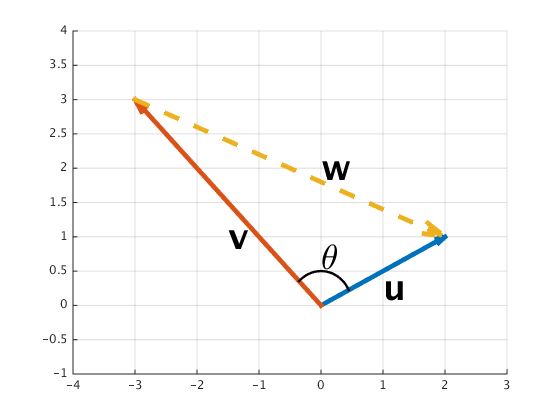
\includegraphics[scale=0.5]{F11_06.png}
\end{center}
\newpage
Låt oss nu beräkna vinkeln: Cosinussatsen ger oss:

\[
    \norm{\vec{w}^2} = \norm{\vec{u}^2} + \norm{\vec{v}^2} - 2 \cdot \norm{\vec{u}} \cdot \norm{\vec{v}} \cdot \cos{{\theta}}
\]
Låt oss bryta ut $\cos{\theta}$
\[
    \cos{\theta} = \frac{\norm{\vec{w}^2} - \norm{\vec{u}^2} - \norm{\vec{v}^2}}{-2 \cdot \norm{\vec{u}} \cdot \norm{\vec{v}}} = \frac{29 - 5 - 18}{2 \cdot \sqrt{5} \cdot \sqrt{18}} = \frac{-1}{\sqrt{10}}
\]
Vilket ger vinkeln $\theta \approx 108^o$
\end{Ex}



% section vektorer (end)


\end{document} 






















